\section{Executing a command from the GUI to the device and back}

To transport data between the real wireless device and the GUI multiple communication instances are involved. The complexity of this communication chain shall be 
explained in the following example:

\begin{figure} 
\begin{center}
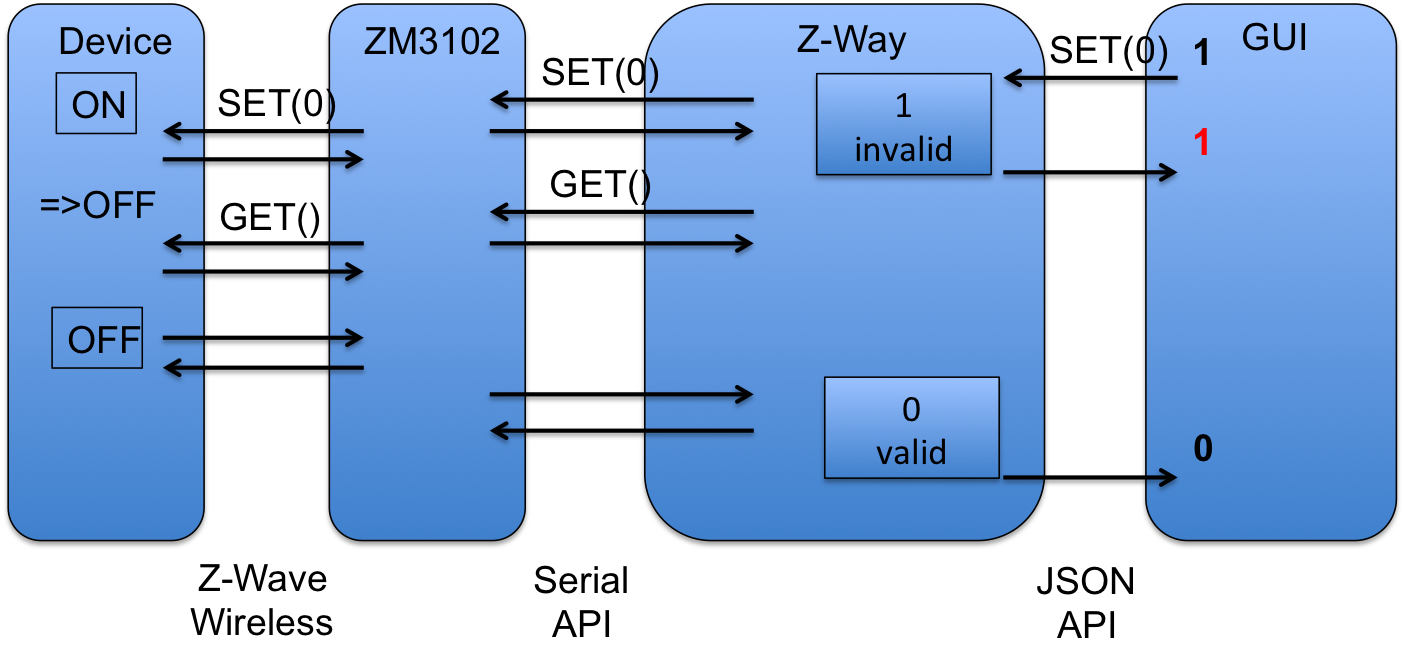
\includegraphics[scale=0.6]{pics/zway2en.png}
\caption{Z-Way Timings}
\label{zwaytimings} 
\end{center} 
\end{figure}

Assuming the GUI shows the status of a remote switch and allows to change the switching state of this device. When the user hits the switching button he expects to 
see the result of his action as a changing status of the device in the GUI. The first step is to hand over the command (SET)  from the GUI to Z-Way using the JSON interface.
Z-Way receives the command and will confirm the reception to the GUI. Z-Way recognizes that the execution of the switching common will likely result in a change 
of the status variable However Z-Way will not immediately change the status variable but invalidate the actual value. This is the correct action because at the moment
when the command was received the status is the remote device has not been changed yet but the status of the switch is now unknown.
If the GUI polls the value it will still see the old value but marked as invalid.
Z-Way will not hand over the switching command to the Z-Wave transceiver chip. Since it is possible that there are other command waiting for execution (sending) by 
the Z-Wave transceiver chip the job queue is queuing them and will handle certain priorities if needed. Z-Way has recognized that the command will likely change the status
of the remote device and is therefore adding another command to call the actual status after the switching command was issued.
The transceiver is confirming the reception of the command and this confirmation is noted in the job queue. This confirmation however only means that the transceiver 
has accepted the command and does neither indicate that the remote device has receives it nor even confirming that the remote device has executed accordingly.
The transceiver will now try to send the commend wirelessly to the remote device. A successful confirmation of the reception from the remote device is the only valid 
indicator that the remote device has received the command (again, not that it was executed!).
The second command (GET) is now transmitted the very same way and confirmed by the remote device. This device will now sent a REPORT command back to Z-Way
reporting the new status of the switching device. Now the transceiver of Z-Way has to confirm the reception. The transceiver will then send the new value to the Z-Way 
engine by issuing a commas via the serial interface. Z-Way receives the report and will update the switching state and validate the value.
From now on the GUI will receive a new state when polling.
